\documentclass[preprint,11pt,authoryear]{elsarticle}
\pdfoutput=1
\pdfminorversion=4 %had problems submitting a v1.5 pdf file with J Neurosci Methods
\usepackage{graphicx}
\usepackage{amsmath}
\usepackage{esint}
\usepackage{amssymb}
\usepackage{lineno}
\usepackage[T1]{fontenc}
\usepackage[utf8]{inputenc}
\usepackage[english]{babel}
\usepackage[]{algorithm}
\usepackage[noend]{algpseudocode}
%% natbib.sty is loaded by default. However, natbib options can be
%% provided with \biboptions{...} command. Following options are
%% valid:

%%   round  -  round parentheses are used (default)
%%   square -  square brackets are used   [option]
%%   curly  -  curly braces are used      {option}
%%   angle  -  angle brackets are used    <option>
%%   semicolon  -  multiple citations separated by semi-colon
%%   colon  - same as semicolon, an earlier confusion
%%   comma  -  separated by comma
%%   numbers-  selects numerical citations
%%   super  -  numerical citations as superscripts
%%   sort   -  sorts multiple citations according to order in ref. list
%%   sort&compress   -  like sort, but also compresses numerical citations
%%   compress - compresses without sorting
%%
%% \biboptions{comma,round}

% \biboptions{}

\bibliographystyle{elsarticle-harv}
\biboptions{square}

\renewcommand\familydefault{\sfdefault}
\usepackage[scaled]{helvet}

\usepackage{units}
\usepackage[usenames, dvipsnames]{xcolor}

\usepackage{soul}
\usepackage{placeins}

\usepackage{nameref}
\usepackage[pdftex,breaklinks=true,colorlinks=true,linkcolor=blue,citecolor=blue,urlcolor=blue,filecolor=blue,pdffitwindow,backref=true,pagebackref=false,bookmarks=true,bookmarksopen=true,bookmarksnumbered=true]{hyperref}
\usepackage[plain]{fancyref}
\usepackage{array}
\usepackage{multirow}

% Text layout
%\hoffset 2 cm
\topmargin 0.0cm
\oddsidemargin 0.5cm
\evensidemargin 0.5cm
\textwidth 16cm 
\textheight 21cm

%custom color for \hlc
\newcommand{\hlc}[2][yellow]{ {\sethlcolor{#1} \hl{#2}} }
\newcommand{\hlb}[2][blue]{ {\sethlcolor{#1} \hl{#2}} }
\newcommand{\hlr}[2][Maroon]{ {\sethlcolor{#1} \hl{#2}} }
\newcommand{\hlj}[2][OliveGreen]{ {\sethlcolor{#1} \hl{#2}} }
\newcommand{\hlR}[2][red]{ {\sethlcolor{#1} \hl{#2}} }

%boxes and highlight color for text updates, personified!
\newcommand{\ghnote}[1]{\color{white}{\hlb{GH: #1 }}\color{black}}
\newcommand{\ghtxt}[1]{{\color{blue}#1}}
\newcommand{\gtenote}[1]{\color{white}{\hlR{GTE: #1 }}\color{black}}
\newcommand{\gen}[1]{\color{white}{\hlR{GTE: #1 }}\color{black}}
\newcommand{\gtetxt}[1]{{\color{red}#1}}
\newcommand{\gex}[1]{{\color{red}#1}}
\newcommand{\genn}[1]{{\color{orange}#1}}

\newcommand{\tvnnote}[1]{\color{white}{\hlj{TVN: #1 }}\color{black}}
\newcommand{\tvntxt}[1]{{\color{OliveGreen}#1}}

%fancy ref formatting
\Frefformat{plain}{\fancyreffiglabelprefix}{Fig~#1}
\newcommand*{\Frefsecshortname}{Section}%
\Frefformat{plain}{\fancyrefseclabelprefix}{\Frefsecshortname~#1}
\Frefformat{plain}{\fancyrefeqlabelprefix}{Eq~(#1)}

%tables as in Nordlie et al. (2009)
\usepackage{tabularx}
\usepackage{colortbl}
\usepackage{morefloats}

%table formatting
\newcommand{\modelhdr}[3]{%
   \multicolumn{#1}{|l|}{%
     \color{white}\cellcolor[gray]{0.0}%
     \textbf{\makebox[0pt]{#2}\hspace{0.5\linewidth}\makebox[0pt][c]{#3}}%
   }%
}
\newcommand{\parameterhdr}[3]{%
   \multicolumn{#1}{|l|}{%
     \color{black}\cellcolor[gray]{0.8}%
     \textbf{\makebox[0pt]{#2}\hspace{0.5\linewidth}\makebox[0pt][c]{#3}}%
   }%
}
\def\tabspace{0.5ex}

\usepackage{float}
\floatstyle{plaintop}
\restylefloat{table}

\journal{nobody}


% redefinition of \author{•} because of bug (reset of \@corref missing), taken from:
% http://tex.stackexchange.com/questions/116515/elsarticle-frontmatter-corresponding-author
%
\makeatletter
\def\@author#1{\g@addto@macro\elsauthors{\normalsize%
    \def\baselinestretch{1}%
    \upshape\authorsep#1\unskip\textsuperscript{%
      \ifx\@fnmark\@empty\else\unskip\sep\@fnmark\let\sep=,\fi
      \ifx\@corref\@empty\else\unskip\sep\@corref\let\sep=,\fi
      }%
    \def\authorsep{\unskip,\space}%
    \global\let\@fnmark\@empty
    \global\let\@corref\@empty  %% Added
    \global\let\sep\@empty}%
    \@eadauthor={#1}
}
\makeatother

% - mine pakker -
\usepackage[exponent-product = \cdot]{siunitx}
\usepackage[colorinlistoftodos]{todonotes}
\usepackage[normalem]{ulem} % strikethroughs \sout{Hello World}
\usepackage{caption}
\usepackage{booktabs} % to make nice tables
\graphicspath{{Figures/}} %Setting the graphicspath
\usepackage{caption}
\usepackage{subcaption}

% - mine kommandoer - 


\begin{document}

\begin{frontmatter}

%% Title, authors and addresses

\title{Computing extracellular electrical potentials from neuronal simulations} 

%% use the tnoteref command within \title for footnotes;
%% use the tnotetext command for the associated footnote;
%% use the fnref command within \author or \address for footnotes;
%% use the fntext command for the associated footnote;
%% use the corref command within \author for corresponding author footnotes;
%% use the cortext command for the associated footnote;
%% use the ead command for the email address,
%% and the form \ead[url] for the home page:
%%
%% \title{Title\tnoteref{label1}}
%% \tnotetext[label1]{}
%% \author{Name\corref{cor1}\fnref{label2}}
%% \ead{email address}
%% \ead[url]{home page}
%% \fntext[label2]{}
%% \cortext[cor1]{}
%% \address{Address\fnref{label3}}
%% \fntext[label3]{}

%% use optional labels to link authors explicitly to addresses:
%% \author[label1,label2]{<author name>}
%% \address[label1]{<address>}
%% \address[label2]{<address>}

\author{Geir Halnes\fnref{label1,label2}}
\author{Torbj\o{}rn V. Ness \fnref{label1}}
\author{Solveig N\ae{}ss\fnref{label2}}
\author{Klas Pettersen \fnref{label3}}
\author{Gaute T. Einevoll\corref{cor1}\fnref{label1,label2,label4}}

\address[label1]{Faculty of Science and Technology, Norwegian University of Life Sciences, {{\AA}}s, Norway}
\address[label2]{Center for Integrative Neuroplasticity, University of Oslo, Oslo, Norway}
\address[label3]{Norwegian Artificial Intelligence Research Consortium, Oslo, Norway}
\address[label4]{Department of Physics, University of Oslo, Oslo, Norway}

\cortext[cor1]{correspondence: \href{geir.halnes@nmbu.no}{gaute.einevoll@nmbu.no}}

%%%%%%%%%%%%%%%%%%%%%%%%%%%%%%%%%%%%%%%%%%%%%%%%%%
%%%%%%%%%%%%%%%%%%%%%%%%%%%%%%%%%%%%%%%%%%%%%%%%%%


\begin{abstract}
%% Text of abstract
\ghnote{Vet ikke hva forfatterordningen skal vaere, men vi faar se det an etter hvert, og bestemme utifra hvem som har jobbet mest med manus. For oeyeblikket leder jeg, men jeg tror jeg satser paa at kanskje Torbjoern fosser forbi etter hvert.}
\tvnnote{Just to be sure: If we make figures for this chapter, we have the right to re-use those wherever we like?}
\tvnnote{Giugliano: max 15-20 pages, by February 2020 }
\end{abstract}

\begin{keyword}
extracellular potentials \sep LFP \sep EEG \sep ECoG \sep electrodiffusion
%% keywords here, in the form: keyword \sep keyword

%% MSC codes here, in the form: \MSC code \sep code
%% or \MSC[2008] code \sep code (2000 is the default)
\end{keyword}

\end{frontmatter}

\tableofcontents

%%%%%%%%%%%%%%%%%%%%%%%%%%%%%%%%%%%%%%%%%%%%%%%%%%
%%%%%%%%%%%%%%%%%%%%%%%%%%%%%%%%%%%%%%%%%%%%%%%%%%
%% Start line numbering here if you want
\linenumbers

\section{Introduction}
\label{sec:introduction}

\ghnote{First something about why we are interested in electrical fields and some historical perspectives. Perhaps Gaute should write this.}

\ghnote{End intro with bridge to theory-section. Probably we should add some older references to VC-theory?}


Very important to model what you measure, and measure what you model \citep{Einevoll2019, Maki-marttunen2019}


Within the field of computational neuroscience, there has been a strong focus on modelling the membrane potential dynamics of morphologically complex neurons. Such simulations involve computing the transmembrane currents in all neuronal segments. This book chapter explains how one, based on knowing the transmembrane currents, can compute the electrical potential in the extracellular space surrounding the active neurons. 

The link between membrane currents and the extracellular potential is of course mediated by electrical currents. Electrical currents in the brain are mediated by the movement of ions, and it is these currents that a recording electrode pick up.  A net electrical current through the extracellular space of the brain could in principle include several components, such as (1) a drift component (ions migrate in electrical fields), (2) a diffusion component (ions diffuse), (3) an advective component (extracellular fluid flow drags ions along), and (4) a displacement component (ions pile up and changes the local charge density). Since the extracellular bulk fluid has very fast relaxation times and is very close to electroneutral, the latter two current components (3-4) are extremely small and are typically neglected \citep{Grodzinsky2011, Gratiy2017}. The diffusive component (3) is acknowledged to play an important role for voltage dynamics on a tiny spatial scale, such as in synaptic clefts or in the close vicinity of neuronal membrane, where ion concentrations can change dramatically within very short time \citep{Savtchenko2017, Pods2017}. At the level of tissue, it is commonly believed that the diffusive current is much smaller than the drift current, so that even diffusive currents are typically neglected \citep{Holt1999, Pettersen2008a}. This is often a useful approximation, since modeling of electrodiffusive processes is computationally expensive and may not be feasible for large and complex systems. However, if concentration gradients are present, diffusive currents could in principle affect measurable extracellular potentials \citep{Halnes2016, Halnes2017, Solbra2018}, and in scenarios involving dramatic shifts in extracellular concentrations, such as spreading depression and related pathologies, diffusive effects are likely to be of key importance for shaping the extracellular potential \citep{Almeida2004, OConnell2016}.

We start this book chapter by giving an overview of the theory used for forward modellng of extracellular potentials, and introduce the mathematical frameworks and software tools that can be used for such modelling. We start the theory-part at the rather fundamental level of electrodiffusive ion concentration dynamics, and derive an electrodiffusive framework for predicting the dynamics of the extracellular ion concentrations and potential. We next show how this theory can be reduced to the simpler, and more common VC-theory if we assume that the diffusive component is negligible. 

\begin{figure}[!ht]
\begin{center}
\includegraphics[width=0.8\textwidth]{cortex_multipop_arial_font}
\end{center}
\caption{\textbf{LFP, ECoG, EEG and MEG.} The same basic building blocks, that is, currents caused by large numbers of synaptic input are contributing to several different measurable signals.}
\label{fig:multimodal}
\end{figure}

Motivation: Simulated test-data for benchmarking
Spike-sorting: \cite{Hagen2016, Buccino2019}, CSD: \cite{Pettersen2006, Potworowski2012, Ness2015}, 
Location and Cell type: \citep{DelgadoRuz2014, Buccino2018}, 
LPA

\section{%Theory: 
From electrodiffusion to volume conductor theory}
\label{sec:theory}
We start at the very smallest of scales considered in neuroscience, by describing the fundamentals of how ions are moving through the brain under the influence of electric fields and concentration gradients. Building on this, we describe how ionic currents affect the electric extracellular potentials inside neural tissue, like the local field potential (LFP), and furthermore, how they cause electric potentials and magnetic fields that are measurable even outside the of the head.

\subsection{Ion concentration dynamics}
\label{sec:eldiff}
In electrodiffusive processes, the flux density of an ion species $k$ is given by \cite{Koch1999}:
\begin{equation}
{\bf J_k} = - D_{k} {\bf \nabla} c_{k} - \frac{D_k z_k c_k}{\psi} {\bf \nabla} \phi,
\label{eq:JNP}
\end{equation}
where the first term on the right is Fick's law for the diffusive flux density $J_{k}^\text{diff}$, and the second term is the drift flux density $J_{k}^\text{drift}$, which expands Fick's law in the case where the diffusing particles also move due to electrostatic forces with a mobility $D_k/\psi$ (cf. the Einstein-relation \cite{Mori2008}). Here $D_{k}$ is the diffusion coefficient of ion species $k$, $\phi$ is the electric potential, $z_{k}$ is the valency of ion species $k$, and $\psi=RT/F$ is defined by the gas constant ($R$), Faraday's constant ($F$)  and the temperature ($T$). The ion concentration dynamics of a given species is then given by the Nernst-Planck continuity equation:

\begin{equation}
\frac{\partial c_k}{\partial t} = - {\bf \nabla} \cdot {\bf J_k} + f_k = {\bf \nabla} \cdot \left[ D_k {\bf \nabla} c_k + \frac{D_k z_k c_k}{\psi} {\bf \nabla} \phi \right] + f_k
\label{eq:NP}
\end{equation}
where $f_k$ represents any source term in the system, such as e.g., an ionic transmembrane current source   \cite{Solbra2018}. 

In order the solve a set (i.e., one for each ion species present) of equations like (\ref{eq:NP}), one needs an expression for the electrical potential $\phi$. There are two main approaches to this. The physically most detailed approach is to use the Poisson-Nernst-Planck (PNP) formalism \citep{Leonetti1998, Leonetti2004, Lu2007, Lopreore2008, Nanninga2008, Pods2013, Gardner2015}. Then $\phi$ is determined from Poisson's equation from electrostatics, 
\begin{equation}
\nabla^2 \phi = -\rho/\epsilon, 
\label{eq:poisson}
\end{equation}
where $\epsilon$ is the permittivity of the system, and $\rho$ is the charge density associated with the ionic concentrations, as given by:
\begin{equation}
\rho = F \sum_k z_k c_k.
\label{eq:F}
\end{equation}
An alternative, more computationally efficient approach is to replace the Poisson equation with the simplifying approximation that the bulk solution is electroneutral \citep{Mori2008, Mori2009, Mori2009a, Mori2011, Halnes2015, Halnes2013, Halnes2015arxiv, Pods2017, Niederer2013, OConnell2016, Solbra2018}, which is a good approximation on spatiotemporal scales larger than micrometers and microseconds \citep{Grodzinsky2011, Pods2017, Solbra2018}. 

Both the PNP formalism and the electroneutral formalism allow us to compute the dynamics of ion concentrations and the electrical potential in the extracellular space of neural tissue containing an arbitrary set of neuronal and glial current sources. For example, in a recent work, a version of the electroneutral formalism was developed into a framework for computing the extracellular dynamics (of $c_k$ and $\phi$) in a 3D space surrounding morphologically complex neurons simulated with the NEURON simulation tool \citep{Solbra2018}. However, both the PNP and electroneutral formalisms keep track of the spatial distribution of ion concentrations, and as such they require a suitable meshing of the 3D space, and numerical solutions based on finite difference- or finite element methods. In both cases, simulations can become very heavy, and for systems at a tissue level, the computational demand may become incommensurable. For that reason, there is much to gain from deriving simpler frameworks where effects of ion concentration dynamics are neglected, since, for many scenarios, this may be a good approximation. Below, we will derive these simpler frameworks using the Nernst-Planck fluxes (eq. \ref{eq:JNP}) as a starting point, as this approach will make the involved approximations transparent.

\subsection{Electrodynamics}
If we multiply eq. \ref{eq:JNP} by $F\cdot z_k$ and take the sum over all ion species, we get an expression for the net electrical current density due to all particle fluxes:

\begin{equation}
{\bf I} = - \sum_k{F z_k D_{k}{\bf \nabla} c_{k}} - \sigma {\bf \nabla}{\phi}
\label{eq:INP}
\end{equation}
where the first term is the diffusive current density $I^\text{diff}$ and the second term is the drift current density$I^\text{drift}$. We have here identified the conductivity $\sigma$ of the medium as \citep{Koch1999}:
\begin{equation}
\sigma = F\sum_{k} \frac{\tilde{D}_{k} z_{k}^2}{\psi}c_{k}.
\label{eq:sigma}
\end{equation}
Current conservation in the extracellular space implies that:
\begin{equation}
{\bf \nabla} \cdot {\bf I} = - \sum_k{F z_k D_{k}\nabla^2 c_{k}} - {\bf \nabla} \cdot (\sigma {\bf \nabla} \phi) = - CSD,
\label{eq:CSD}
\end{equation}
where $CSD$ denotes the current source density, reflecting e.g., local neuronal or glial transmembrane currents. We note that this is essentially equivalent to eq. \ref{eq:NP} at the level of single ion species, with the exception eq. \ref{eq:NP} contained a term $\partial c_k/ \partial t$ for accumulation of ion species $k$, while eq. \ref{eq:CSD} does \emph{not} contain a corresponding term ($\partial \rho/ \partial t$) for charge accumulation. Hence, in eq. (\ref{eq:CSD}) it is implicitly assumed that the extracellular bulk solution is electroneutral \citep{Solbra2018}. We note that in general, the $CSD$ term includes both ionic transmembrane currents and transmembrane capacitive currents, and that the latter means that the local charge accumulation building up the transmembrane potential still occurs in the membrane Debye-layer.

Note that if we assume all concentrations to be constant in space, the diffusive term vanishes, and eq. (\ref{eq:CSD}) reduces to:
\begin{equation}
{\bf \nabla} \cdot (\sigma {\bf \nabla} \phi) = - CSD,
\label{eq:CSDstandard}
\end{equation}
This the standard expression used in current source density (CSD) theory \citep{Mitzdorf1985, Nicholson1975, Pettersen2006}, where spatially distributed recordings of $\phi$ are used to make theoretical predictions of underlying current sources. When using Eq. \ref{eq:CSDstandard}, it is implicitly assumed that the Laplacian of $\phi$ exclusively reflects transmembrane current sources, and that it is not contributed to by diffusive processes. 

As eq. (\ref{eq:CSD}) indicates, also diffusive processes can in principle contribute to the Laplacian of $\phi$, and if present, they could give rise to a non-zero Laplacian of $\phi$ even in the absence of neuronal sources ($CSD = 0$). Previous computational have predicted that effects of diffusion on extracellular potentials are not necessarily small, but tend to be very slow, meaning that they will only affect the very low-frequency components of $\phi$ \citep{Halnes2016, Halnes2017}. This is due to the diffusive current being a direct function of ion concentrations $c_k$, which on a large spatial scale typically vary on a much slower time scale (seconds-minutes) than the fluctuations in $\phi$ that we commonly are interested in (milliseconds-seconds). Furthermore, electrodes used to record $\phi$ typically have a lower cutoff frequency of 0.1-1Hz \citep{Einevoll2013}, which means that most of the tentative diffusive contribution will be filtered out from experimental recordings. It may therefore be a good approximation to neglect the diffusive term, except in the case of pathologically dramatic concentration variations. For the rest of this chapter, we shall do so, and assume that electrodynamics in neural tissue can be determined by eq.~(\ref{eq:CSDstandard}).

\subsection{Volume conductor theory}
\label{sec:VC_theory}
In simulations of morphologically complex neurons, we typically compute a set of transmembrane current sources for each neuronal segment \citep{Koch1999}. Commonly, one assumes that the extracellular potential does not effect the neurons (i.e., no ephaptic coupling), since extracellular potentials are typically much smaller than the membrane potential of $\sim$-70~mV. 
By assuming that the tissue medium is a volume conductor \citep{Holt1999, Linden2014},  one can then use the standard CSD-equation (eq. \ref{eq:CSDstandard}) to perform a forward modeling of the extracellular potential at each point in space surrounding the neuron(s). 

For the simplest case of a single point source $I_1$ at a point ${\bf r}=0$ in an isotropic medium, the solution is: 

\begin{equation}
\phi = \frac{I_1}{4\pi \sigma r },
\label{eq:pointsource}
\end{equation}
\tvnnote{I think we should explain where $4\pi r$ comes from}
where $r$ is the distance from the source. With several point-current sources, $I_{1}, I_2, I_3, ... $ in locations ${\bf r_1}, {\bf r_2}, {\bf r_3} ... $, we can apply the superposition principle\tvnnote{Refer to linearity assumption}, and the potential in a point ${\bf r}$ is given by:

\begin{equation}
\phi({\bf r}) = \frac{I_1}{4\pi  \sigma {\bf |r-r_1|}} + \frac{I_2}{4\pi  \sigma {\bf |r-r_2|} } + \frac{I_3}{4\pi  \sigma {\bf |r-r_3|} } + ... = \sum_k \frac{I_k}{4\pi  \sigma {\bf |r-r_k|} }.
\label{eq:VCtheory}
\end{equation}

Eq.~\ref{eq:VCtheory} is often referred to as the point-source approximation \citep{Holt1999, Pettersen2008a}, since the membrane current from a neuronal segment is assumed to enter the extracellular medium in a single point. An often used further development is obtained by integrating eq.~\ref{eq:VCtheory} along the segment axis, corresponding to the transmembrane current being evenly distributed along the segment axis, giving the line-source approximation \citep{Holt1999, Linden2014}.

The formula in eq. \ref{eq:VCtheory} (or the line-source version of it) represents volume conductor theory in its simplest form, and was based on a set of assumptions, some of which may be relaxed for problems where it is relevant: 

\begin{enumerate}

\item {\bf Quasi-static approximation of Maxwell's equations:} Terms with time derivative of the electrical and magnetic fields are neglected. This approximation appears to be well-justified for the relatively low frequencies relevant for brain signals, below about 10 kHz \citep{Nunez2006}.

\item {\bf Linear extracellular medium:} Linear relationship ($\bf{I} = -\sigma {\nabla \phi}$) between the current density ${\bf I}$\tvnnote{I would have preferred J to mean current density and I total currents. Will this make things messy other places?} \ghnote{Maybe it messes things up, since I used $J_k$ for fluxes earlier.} \tvnnote{Hmm, im my mind current density and flux was the same thing?} and the electrical field, $\nabla \phi$. This is essentially Ohm's law for volume conductors, and the relation is constitutive, meaning that it is observed in nature rather than derived from any physical principle \citep{Nunez2006, Pettersen2012}.

\item {\bf Frequency independent conductivity:} Capacitive effects in neural tissue are assumed to be negligible compared to resistive effects in volume conduction. This approximation seems to be justified for the relevant frequencies in extracellular recordings \cite{Logothetis2007, Miceli2017, Ranta2017}, but it is possible to expand the formalism to include a frequency dependent conductivity \citep{Tracey2011, Miceli2017}. See Fig.~\ref{fig:freq_dep}.

\item {\bf Isotropic conductivity:} The electrical conductivity, $\sigma$, was assumed to be the same in all spatial directions. This is mostly an acceptable approximation, but it is also possible to expand the formalism to account for an anisotropic conductivities \citep{Ness2015}. \ghnote{Referere til et senere kapittel der vi bruker dette.}

\item {\bf Homogeneous  conductivity:} The extracellular medium was assumed to have the same conductivity everywhere. Although neural tissue is highly non-homogeneous on the micrometer scale \citep{Nicholson1998}, microscale inhomogeneities may average out on a larger spatial scale, and a homogeneous conductivity seems to be a reasonable approximation within cortex \citep{Logothetis2007}. However, in many situations is will not be applicable, and in general, eq.~\ref{eq:CSDstandard} can always be solved for arbitrarily complex geometries using numerical methods, like the Finite Element Method (FEM) \citep{Logg2012}. For some example neuroscience applications, see \cite{Moffitt2005, Frey2009, Joucla2012, Haufe2015, Ness2015, Buccino2019b, Obien2019}. For some simple non-homogeneous cases analytical solutions can still be obtained, for example through the Method of Images for {\it in vitro} brain slices \citep{Ness2015}, and the four-sphere head model for EEG signals (Sec.~\ref{sec:EEG}) \citep{Naess2017}. \ghnote{Antar at vi her refererer til EEG-kapittelet og evt. flytter noe av dette materialet dit?}
\tvnnote{Kun siste del-setning som spesifikt handler om EEG, i tillegg til noen av referansene.}

\item {\bf No diffusion:} To account for diffusion, one would need to compute the electrodynamics of the system using one of the electrodiffusive frameworks presented in Section \ref{sec:eldiff}.

\end{enumerate}


\begin{figure}[!ht]
\begin{center}
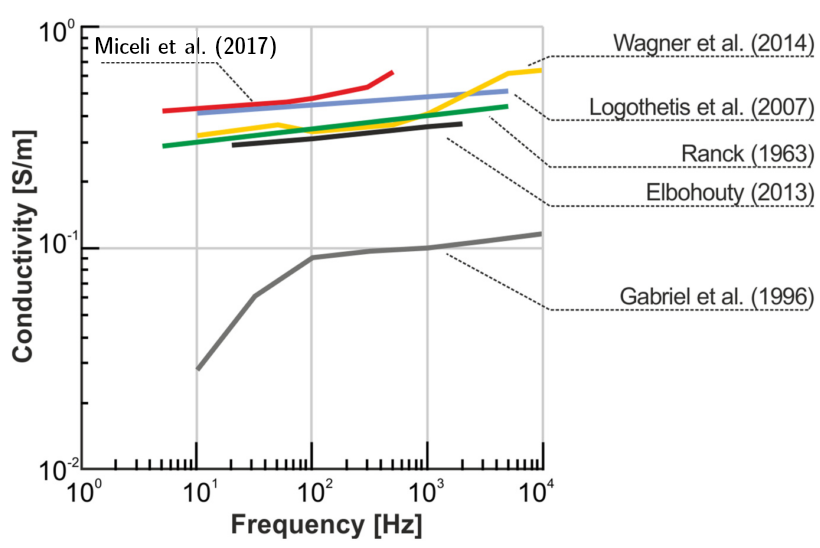
\includegraphics[width=0.6\textwidth]{frequency_dependence}
\end{center}
\caption{\textbf{Literature review of reported conductivities in various species and experimental setups.} 
Gabriel et al. (1996): data from bovine brains recorded with a two-electrode setup. Elbohouty (2013): data recorded in vitro in slices of mouse cerebral cortex with a two-electrode setup. Logothetis et al. (2007): data from monkey recorded with a four-electrode setup. The average conductivity value, 0.405 S/m, combined with the reported increase of $\sim$25\%. Wagner et al. (2014): recordings from cat cerebral cortex with a two-electrode setup, which was similar to the setup used by Gabriel et al. (1996). Ranck (1963): data from rabbit brain.
}
\label{fig:freq_dep}
\end{figure}



Volume conductor theory is the fundament for forward modeling of extracellular potentials at different spatial scales, from extracellular spikes, LFPs and MUAs, to ECoGs and EEGs. In the following sections we shall review previous modeling works, and insights from simulating electrical potentials at these different scales.
We use the software LFPy \citep{Linden2014, Hagen2018, Hagen2019}, which has volume conductor theory incorporated and can in principle be used to compute extracellular potentials on arbitrarily large spatial scales, surrounding arbitrarily large neuronal populations. 


\section{Single-cell contributions to extracellular potentials}
%\ghnote{Suggest that we start these sections by explaining what $\phi$ tells us at this level. Also, we should refer to the VC-theory and explain which of the assumptions (1-6) that were relaxed in the specific case.}

%\ghnote{Maybe not use current-conservation as a main topic, but rather talk about how extracellular potentials reflect morphology. Say something like: The extracellular potential arising from the activity of a single neuron is a reflection of not only its dynamical activity, but also its  morphology, and neurons with a large spatial extension generally give rise to larger extracellular potentials as there will be larger distances between current.}

%\ghnote{Moved current-conservation figure here. I think that we could call it something else. Perhaps the Hay-neuron-example can be integrated with this figure? And perhaps we should name it single-cell contribution to extracellular potential}.

The transmembrane currents of a neuron during some arbitrary neural activity can be used to calculate extracellular potentials, by applying the formalism described in Sec.~\ref{sec:VC_theory}, and in the simplest case eg.~\ref{eq:VCtheory}.
%The extracellular potentials from a single neuron is a reflection of both cellular dynamics and morphology (the spatial structure of the cell). 
Current conservation requires that the transmembrane currents across the entire cellular membrane at any given time sum to zero \citep{Koch1999, Nunez2006}, and since
an excitatory synaptic input generates a current sink (negative current), this will necessarily lead to current sources elsewhere on the cell. This implies that point neurons, that is, neurons with no spatial structure, will have no net transmembrane currents, and hence cause no extracellular potentials (Fig.~\ref{fig:EP_morph}A). The simplest neuron models that are capable of producing extracellular potentials are therefore two-compartment models, which will have two equal but opposite currents, and cause perfectly dipolar extracellular potentials (Fig.~\ref{fig:EP_morph}B).

Multi-compartment neuron models mimicking the complex spatial structure of real neurons will typically give rise to complicated patterns of current sinks and sources (negative and positive currents respectively), leading to complex, but mostly dipolar-like extracellular potentials (Fig.~\ref{fig:EP_morph}C) \citep{Einevoll2013}.
Note that this framework for calculating extracellular potentials is valid both for subthreshold and suprathreshold neural activity, that is, when a cell receives synaptic input that does not trigger, or does trigger an action potential, respectively (Fig.~\ref{fig:EP_morph}, D versus E).  

\begin{figure}[!ht]
\begin{center}
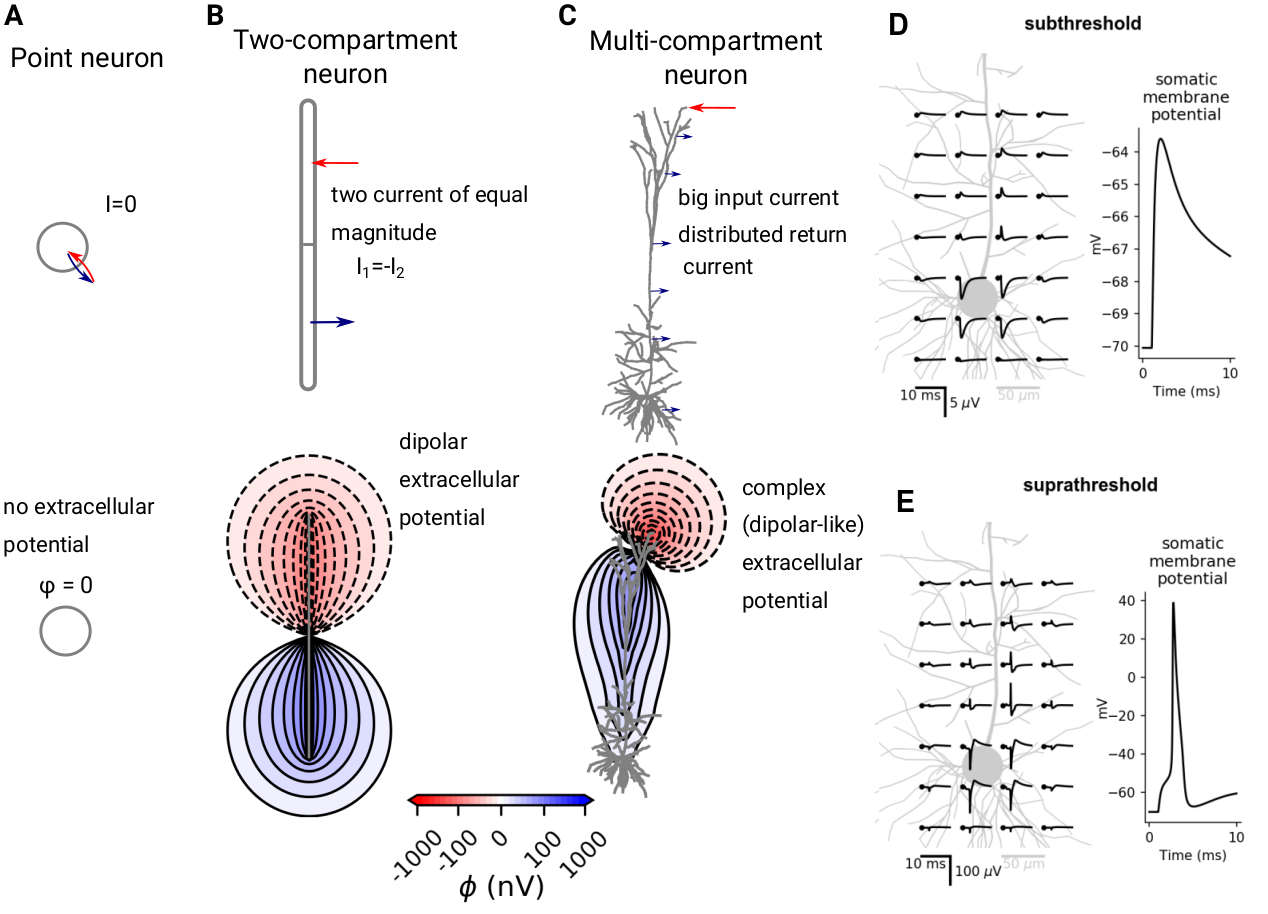
\includegraphics[width=1\textwidth]{single_cell_EP}
\end{center}
\caption{\textbf{Single-cell contributions to the extracellular potential.} 
{\bf A}: Point neurons have no net currents (top), and therefore cause no extracellular potentials (bottom). 
{\bf B}: Two-compartment neuron models have two opposite currents
of identical magnitude (top), and cause perfectly dipolar extracellular potentials (bottom). 
{\bf C}: Multi-compartment neuron models \citep{Hay2011} give rise to complex source-sink patterns (top) and complex (but mostly dipolar-like) extracellular potentials (bottom). 
{\bf D, E}: A single somatic synaptic input to a complex multi-compartment cell model, either subthreshold (D) or suprathreshold (E; double synaptic weight of D), illustrating that the same framework can be used to calculate both the LFP contribution from subthreshold synaptic input, and extracellular action potentials. 
}
\label{fig:EP_morph}
\end{figure}

\section{Intra-cortical measurements from neural populations}
Measured signal often spit in two frequency parts, LFP and MUA. Tell us different things about neural activity.

\subsection{Local field potentials}

% \tvnnote{How much of an intro should we have here? If the Chapter intro has a broader focus and only refer to modelling of brain signals, we should have full LFP intro here.}
% \ghnote{I think we could skim through the different measurement modalities in the intro, and mention LFP, MUA, ECoG and EEG. As of now, there is just a line there, saying that it is very important to model what you measure, and measure what you model.  I suggest that Gaute expands on this, and talks about the needs within the field. However, I suggest that we make it rather brief, and focus this chapter on the technical aspect of how to compute the different measures here.}

The Local Field Potential is the Low-Frequency Part ($\lesssim$ 500~Hz) of the extracellular potentials, and it is among the oldest and most used brain signals in neuroscience \citep{Einevoll2013}. The LFP is expected to be dominated by large numbers of synaptic inputs to populations of geometrically aligned neurons \citep{Nunez2006, Linden2011, Einevoll2013b}.
\tvnnote{Find place to put sentence of two on importance of correlation.}

In cortex and hippocampus, neuron can broadly speaking be divided into two main classes: the inhibitory interneurons, and the excitatory pyramidal neurons. Pyramidal neurons typically have a clear axis of orientation, that is, the apical dendrites of close-by pyramidal neurons tend to be oriented in the same direction (Fig.~\ref{fig:LFP_EEG}A). This geometrical alignment transfers to the current dipoles originating from synaptic input \ghnote{Litt forvirrende setning, dette her} to specific regions of a pyramidal cell population (Fig.~\ref{fig:LFP_EEG}B).  For example, basal excitatory synaptic input generates a current sink and corresponding negative LFP deflection in the basal region, and simultaneously a current source and corresponding positive LFP deflection in the apical region, while apical excitatory synaptic input leads to the reversed pattern (Fig.~\ref{fig:LFP_EEG}C). 
Importantly, this means that excitatory input that simultaneously targets both the apical and the basal dendrite will give opposite source/sink patterns which will lead to substantial cancellation in the LFP (Fig.~\ref{fig:LFP_EEG}C; but see also \cite{Ness2018}).
The same arguments also applies to inhibitory synaptic inputs, with the signs of the currents reversed. 

Note that, for example, the LFP signature of apical excitatory synaptic input is inherently similar to that of basal inhibitory input, and indeed, separating between cases like this pose a real challenge in interpreting LFP signals \citep{Linden2010}. 

In contrast to pyramidal neurons, interneurons often lack any clear orientational specificity, meaning that the current dipoles do not align, leading to negligible contribution to LFP signals, except indirectly through giving synaptic input to pyramidal cells \citep{Hagen2016, Telenczuk2016}.

\begin{figure}[!ht]
\begin{center}
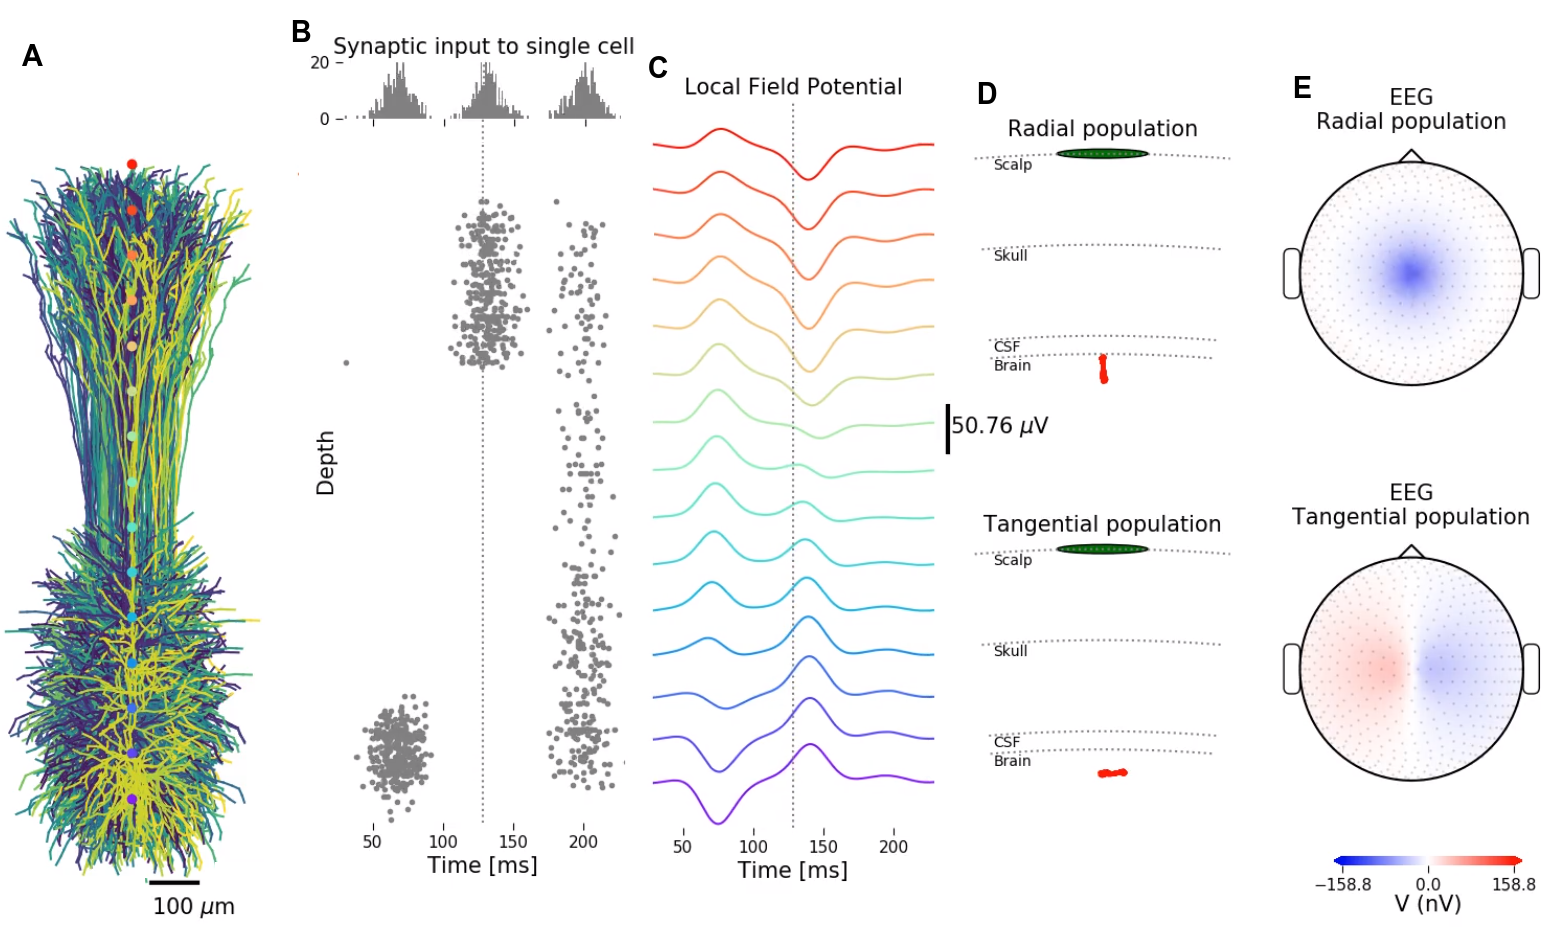
\includegraphics[width=1\textwidth]{population_EEG_MEG.png}
%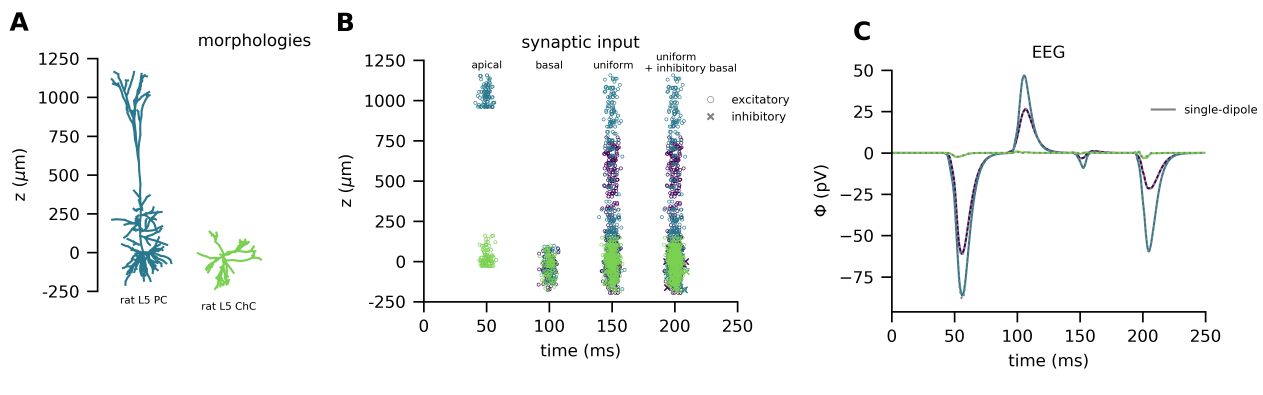
\includegraphics[width=1\textwidth]{PC_versus_IN}
\end{center}
\caption{\textbf{Extracellular potentials from different waves of synaptic input}. Different brain signals from separate waves of synaptic input to 10 000 layer 5 pyramidal cells from rat \citep{Hay2011}.
{\bf A}: A subset of 100 pyramidal cells, with the LFP electrode locations indicated in the center (colored dots).
{\bf B}: Depth-resolved synaptic inputs arrive in three waves, first targeting the basal dendrites (t=$\sim$60~ms), then the apical dendrites (t=$\sim$130~ms), and lastly uniformly across the entire depth (t=$\sim$200~ms). Note that all synaptic input is pre-defined, that is, there is no network activity.
{\bf C}: The LFP at different depths (colors correspond to dots in panel A)
{\bf D}: The four-sphere head model with two orientations of the neural population, either radial, mimicing a population in a gyrus (top) or tangential, mimicing a population in a sulcus (bottom).
{\bf E}: A snapshot of the EEG signal at the head surface for apical input (time marked with dotted line in panel B and C), for a radial population (top) or tangential population (bottom).
}
\label{fig:LFP_EEG}
\end{figure}

%Large spatial extension generally give rise to larger extracellular potentials as there will be larger distances between currents.\tvnnote{Should we derive dipole-formula here, or wait for EEG section? Arguments for having it here: Talk about how large cells gets larger current dipole moments, and how dipoles dominate at larger distances.}

%\ghnote{Forslag som evt. erstatter subsectionen nedenfor:}
%\tvnnote{Tenkte det ble litt ryddigere med underoverskrifter, slik at det er lettere \aa~finne tilbake igjen? Ellers syntes jeg det var en bra omskrivning. }
Although the LFP is believed to predominantly reflect synaptic inputs, active conductances may also contribute to its shaping. Especially slower conductances may play a key role in this, such as long-lasting after-hyperpolarization currents \cite{Reimann2013}, calcium spikes \cite{Suzuki2017}, or the hyperpolarization-activated cation channel I$_{\rm h}$ \cite{Ness2016, Ness2018}. Action potentials are typically expected to contribute little to cortical LFP signals for several reasons \citep{Einevoll2013, Haider2016}, for example, their very short duration with both positive and negative phases (Fig.~\ref{fig:EP_morph}E) would require extreme synchrony to sum constructively in the LFP, and their high frequency content is to a large degree removed from LFPs during low-pass filtering. Note however, that in the hippocampus the highly synchronized spikes found during sharp wave ripples are expected to strongly shape the LFP \citep{Schomburg2012, Luo2018}. 

\subsection{MUA}
While LFPs are thought to mainly reflect the synaptic input to large populations, the multi-unit activity (MUA) can be used to probe the population spiking activity \citep{Pettersen2008}. This can be usefull, as some cell-types, like stellate cells and interneurons are expected to have very weak LFP contributions, but might still be measureable through their spiking activity.
MUA can be used in combination with LFP to estimate the population dynamics, as for example in Laminar Population Analysis \citep{Einevoll2007, Blomquist2009}.
\tvnnote{Not sure what to say about MUA. Could make illustration figures similar to those from Pettersen, Hagen, Einevoll (2008)?} 

\section{ECoG and EEG}
\label{sec:EEG}
LFP signals are measured inside different brain structures, in the immediate vicinity of the current sources that are causing the LFP signals. A disadvantage with this is that it is invasive, in the sense that electrodes must be inserted into the brain tissue which can only be done in humans when there is a clear medical need, like for patients with intractable epilepsy [cite]. However, the current sources that are causing the LFP signals are also causing measurable electrical signals at the brain surface, electrocorticography (ECoG), and outside of the head, called electroencephalograpy (EEG) (Fig.~\ref{fig:multimodal}).

Any combination of current sinks and sources can set up current multipoles \citep{Nunez2006}, and from electrodynamics we know that extracellular potentials at a distance $R$ from the source can be precisely described by a multipole expansion
\begin{equation}
\phi(R) = \frac{C_{monopole}}{R} + \frac{C_{dipole}}{R^2} + \frac{C_{quadrupole}}{R^3} + \frac{C_{octupole}}{R^4} + ...~.
\label{eq:dipole_expansion}
\end{equation}
Since current monopoles are unphysical due to current conservation, and the quadrupole, octupole and higher order terms are decreasing more strongly with distance $R$ than the dipole term, when $R$ is sufficiently large, the extracellular potential from a neuron simulation can be estimated with the \textit{current dipole approximation} \citep{Pettersen2008, Pettersen2014, Nunez2006}:
\begin{equation}
\phi(\mathbf{r}) = \frac{1}{4 \pi \sigma} \frac{|\mathbf{p}| \cos \theta}{R^2}~.
\label{eq:dipole}
\end{equation}
Here, $\mathbf{p}$ is the current dipole moment in a medium with conductivity $\sigma$, $R = |\mathbf{R}|$, where $\mathbf{R}$ is the distance between the current dipole moment and the electrode location and $\theta$ denotes the angle between $\mathbf{p}$ and $\mathbf{R}$. As mentioned above, this approximation is applicable in the far-field limit, that is when $R$ is much larger than the dipole length $d$, $R > 3d$ or $4d$ \citep{Nunez2006}.

\subsection{Head models}
Can use analytic four-sphere (Fig. \ref{fig:head_models}A) \citep{Hagen2018, Naess2017}
Can also used pre-solved complex head models, like the New York head (Fig. \ref{fig:head_models}B) \citep{Huang2016}.

No important signal filtering by head \citep{Pfurtscheller1975, Ranta2017}.


\tvnnote{Write something about the spatial filtering from electrode size.}
\tvnnote{Show extracellular potential through four-sphere head model for single synaptic input to Hay model (same as earlier LFP figure)?}



\begin{figure}[!ht]
\begin{center}
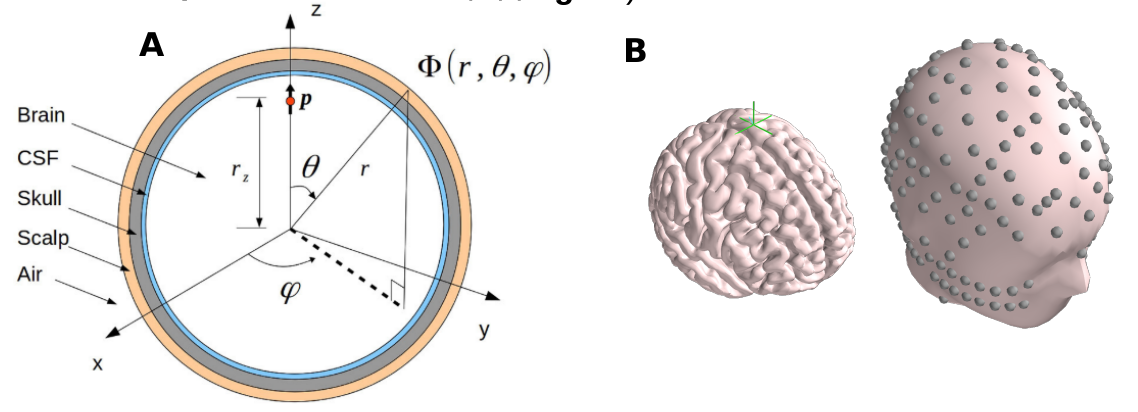
\includegraphics[width=1\textwidth]{head_models.png}
\end{center}
\caption{\textbf{[placeholder] Head models} A: Four-sphere. B: New York head model.}
\label{fig:head_models}
\end{figure}



\section{Other approaches}
Kernels \citep{Hagen2016}

Proxies \cite{Mazzoni2015}

LFP Kernels from experimental spike-triggered averages (Destexhe?)


\section{Other brain signals}
This chapter concerns modelling of extracellular potentials, but the same approach can often be easily extended to also simultaneously calculate other brain signals.

\subsection*{Magnetoencephalograpy (MEG)}
MEG are expected to originate from the same process at LFP, ECoG and EEG signals (Fig.~\ref{fig:multimodal}), that is, synaptic input
to geometically aligned populations of pyramidal neurons, but
is a measure of magnetic instead of electric fields \citep{Hamalainen1993}, and because of the nature of magnetic fields, MEG is most sensitive to populations that are tangential to the head surface, instead of radial (see Fig. \ref{fig:LFP_EEG}D). Except for this difference, much of what is said about electric signals also applies to the magnetic signals.
\subsection*{Voltage-sensitive dye imaging}
In principle easy to model, just area-weighted membrane potential
\subsection*{Calcium imaging}
Depends on cell models with good calcium dynamics, which is a weakness of many present models.
\subsection*{fMRI}
Underlying mechanism for other signals seems clear, but this is not so for fMRI. fMRI is thought to be a measure of ''metabolic cost``, but appears cell-type dependent, with an important role of NPY interneurons.


\section{Software tools}
LFPy etc.
\tvnnote{Recycle text from LFPy 2.0 paper about other softwares (sec 4.7.}
\tvnnote{Maybe we don't need this section? Just say that 'here we've used LFPy'}

Typically split into two separate tasks: Simulate neural activity, mostly relying on the NEURON simulator \citep{Hines1997}, through the Python interface \citep{Hines2009}. Extracellular potentials are then calculated from these currents, through volume conductor theory. 


\section{Summary}
\label{sec:summary}
\begin{enumerate}
 \item Summary of chapter
 \item Ongoing large-scale projects (HBP, Allen)
 \subitem Using LFP in constraining models?
 \item Brain-Machine interfaces?
 \item Where to go?
 \subitem fMRI, VSD, Ca img.
\end{enumerate}



%%%%%%%%%%%%%%%%%%%%%%%%%%%%%%%%%%%%%%%%%%%%%%%%%%
%%%%%%%%%%%%%%%%%%%%%%%%%%%%%%%%%%%%%%%%%%%%%%%%%%

\section*{Acknowledgements}
\label{sec:acknowledgements}
This research has received funding from the European Union Horizon 2020 Framework Programme for Research
and Innovation under Specific Grant Agreement No. 785907 (Human Brain Project SGA2), the Research Council of Norway (Notur, nn4661k), and \tvnnote{INCF?}



%%%%%%%%%%%%%%%%%%%%%%%%%%%%%%%%%%%%%%%%%%%%%%%%%%
%%%%%%%%%%%%%%%%%%%%%%%%%%%%%%%%%%%%%%%%%%%%%%%%%%

\section*{References}
\label{sec:bibliography}
\bibliography{ECS_bookchapter.bib}


%%%%%%%%%%%%%%%%%%%%%%%%%%%%%%%%%%%%%%%%%%%%%%%%%%
%%%%%%%%%%%%%%%%%%%%%%%%%%%%%%%%%%%%%%%%%%%%%%%%%%

\section{Removed}
{\bf Homogeneous:} 
On the spatial scale of a few micrometers, neural tissue is expected to be highly non-homogeneous, consisting of about 20~\% highly conductive cerebrospinal fluid (CSF) \citep{Nicholson1998, Nunez2006} with an electrical conductivity of about 1.5~S/m \citep{Martinsen2008, Logothetis2007, Miceli2017}, and about 80~\% cells, which from the viewpoint of extracellular currents are essentially non-conducting objects. 
The effective conductivity of neural tissue on the macroscale reflects this \citep{Nunez2006}: 20~\% of 1.5~S/m is 0.3~S/m, similar to what is typically measured for the neural tissue conductivity \citep{Logothetis2007, Goto2010, Miceli2017}. 
When deriving the expression for the extracellular potential, we assumed that the described microscale inhomogeneities was averaged out, and that the (effective) conductivity of neural tissue, $\sigma$, was constant. This assumption is expected to be reasonable within cortex, however, in several situations is will not be applicable.

With a spatially varying $\sigma$, we would have to derive the theory from (eq. \ref{eq:CSD} with no diffusive term):
\begin{equation}
CSD = {\bf \nabla}{\bf I} = {\bf \nabla}{\left(\sigma {\bf E}\right)} = - \nabla{\left(\sigma {\bf \nabla} \phi\right)} \\
= -\nabla \sigma \nabla \phi - \sigma \nabla^2 \phi.
\label{eq:poisson_}
\end{equation}

 A frequency dependent conductivity can be incorporated into the forward modelling scheme, essentially by solving eq.~\ref{eq:VCtheory} for each frequency component separately, that is, the transmembrane currents are transformed into the frequency domain by a Fourier Transform, and eq.~\ref{eq:VCtheory} is used with a separate conductivity for each frequency, before the signal is transformed back to the time domain \citep{Tracey2011, Miceli2017}.
Beware however that to preserve causality, that is, no signature of an event should be visible in the extracellular potential before the event has happened, one must also find the appropriate phase-shifts, for example through the Kramers–Kronig relations\citep{Martinsen2008, Miceli2017}.

\subsection*{Single-cell LFP contributions}
Excitatory synaptic inputs opens small pores (ion-channels) in the cellular membrane of the post-synaptic cell, causing positive ions to flow into the cell \citep{Kandel2012}, which, by convention, is referred to as a current sink (negative current). As we have seen, this will necessarily lead to a current source somewhere else on the cell (Sec.~\ref{sec:corrent_conservation}).  
Excitatory synaptic input to the apical dendrite of a pyramidal cell, will tend to give an apical current sink and a corresponding basal current source (Fig.~\ref{fig:dipole_basics}A), while excitatory synaptic input to the basal dendrite will give the opposite: a basal sink and an apical source (Fig.~\ref{fig:dipole_basics}B). Importantly, this means that excitatory input that simultaneously targets both the apical and the basal dendrite will give opposite source/sink patterns which will lead to substantial cancellation, and result in a much weaker contribution to the LFP (Fig.~\ref{fig:dipole_basics}C) (but see \cite{Ness2018}).
The same arguments also applies to inhibitory synaptic inputs, with the signs of the currents reversed (Fig.~\ref{fig:dipole_basics}D-F). 

Note that, for example, the LFP signature of apical excitatory synaptic input is inherently similar to that of basal inhibitory input (Fig.~\ref{fig:dipole_basics}, A versus E), and indeed, separating between cases like this poses a real challenge in interpreting LFP signals [cite]. 

Broadly speaking, neurons can be divided into two main classes: the inhibitory interneurons, and the excitatory pyramidal neurons, which make up about 20~\% and 80~\% of the total neuron numbers respectively \citep{Kandel2012}. While a typical pyramidal neuron has a clear axis of orientation, that is, the apical dendrites of close-by pyramidal neurons tend to be oriented in the same direction, this is much less true for interneurons, which often lack any clear orientational specificity. This has important consequences for their ability to contribute to the LFP: 


\begin{figure}[ht!]
\begin{center}
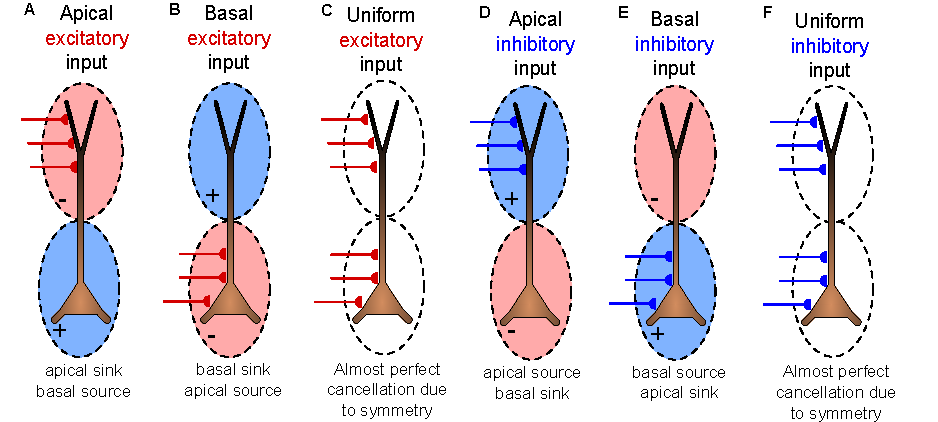
\includegraphics[width=0.8\textwidth]{dipole_basics}
\end{center}
\caption{\textbf{Basic building blocks of the LFP.} Illustration of the LFP at a snapshot in time in a region around a pyramidal cell in response to different types of synaptic input.  
The LFP signature depends on the type of synaptic input (excitatory or inhibitory), and the location (apical, basal, uniform), but also, to a lesser degree, to many other parameters of the cells and synapses.
}
\label{fig:dipole_basics}
\end{figure}

\section{The vital role of current conservation}
\label{sec:corrent_conservation}
Neural simulations with detailed multi-compartment cell models is based on solving the cable equation (Chapter in this book?), with a built-in assumption of current conservation \citep{Koch1999}. Current conservation implies that the summed current across the cellular membrane will, at any given time, sum to zero,
\begin{equation}
 \sum_k I_k = 0.
 \label{eq:current_conservation}
\end{equation}
Note that the capacitive currents have a vital role in ensuring this current conservation: the membrane potential is caused by a slight charge imbalance between the inside and the outside of the cell, and all this surplus charge is expected to be distributed on the cellular membrane, where all the surplus charge on the inside of the cellular membrane (negative during the resting state) is exactly balanced by an equal amount of charge of the opposite polarity on the outside of the cellular membrane (Fig.~\ref{fig:capacitive_currents}A) [cite]. 
As current pass through the membrane, or from one part of the cell to another, the amount of surplus charge on the inside of the cellular membrane changes (Fig.~\ref{fig:capacitive_currents}B), which immediately results in a corresponding change in the amount of charge on the outside of the cellular membrane (Fig.~\ref{fig:capacitive_currents}C). Such changes in the amount of surplus charge distributed along the outside of the cellular membrane are what is called capacitive currents, and they ensure that eq.~\ref{eq:current_conservation} is always fulfilled.
Current conservation has far-reaching consequences for extracellular potentials, that we will illustrate with three examples.
\begin{figure}[ht!]
\begin{center}
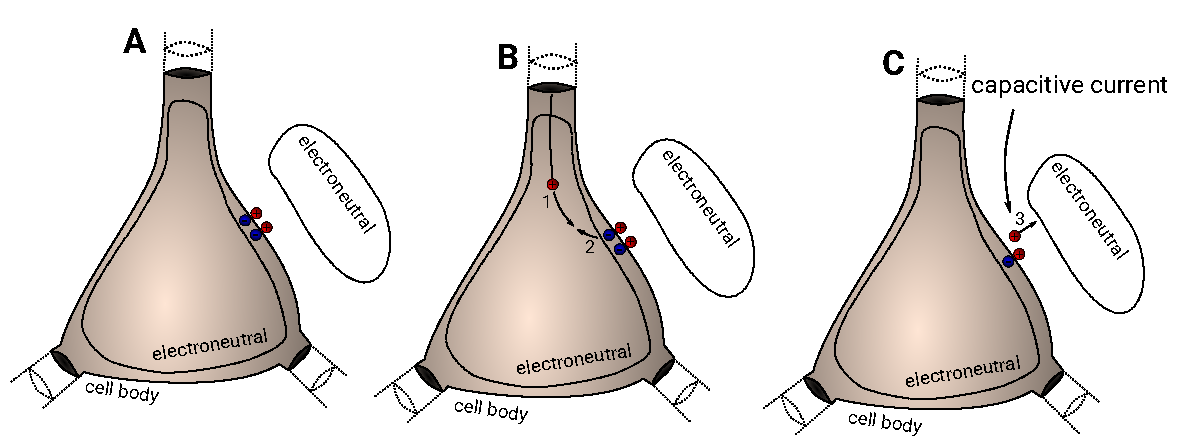
\includegraphics[width=1\textwidth]{capacitive_currents}
\end{center}
\caption{\textbf{Capacitive currents ensures current conservation.
\tvnnote{Mention time scale of this?}
\tvnnote{Not sure if this makes sense to include?}
}}
\label{fig:capacitive_currents}
\end{figure}

\subsection*{Illustration with point-neuron model}
Consider for example the often-used point-neuron models \citep{Sterratt2011}. Since they have only one compartment, eq.~\ref{eq:current_conservation} demands that there should be no net transmembrane current, implying no extracellular potentials (see eq.~\ref{eq:VCtheory}). This means that, while point-neurons have an important role to play in investigating neural network dynamics \citep{Einevoll2019}, they are in general incapable of producing extracellular potentials (Fig.~\ref{fig:EP_morph}A; see however \cite{Mazzoni2015, Hagen2016}). 

\begin{figure}[ht!]
\begin{center}
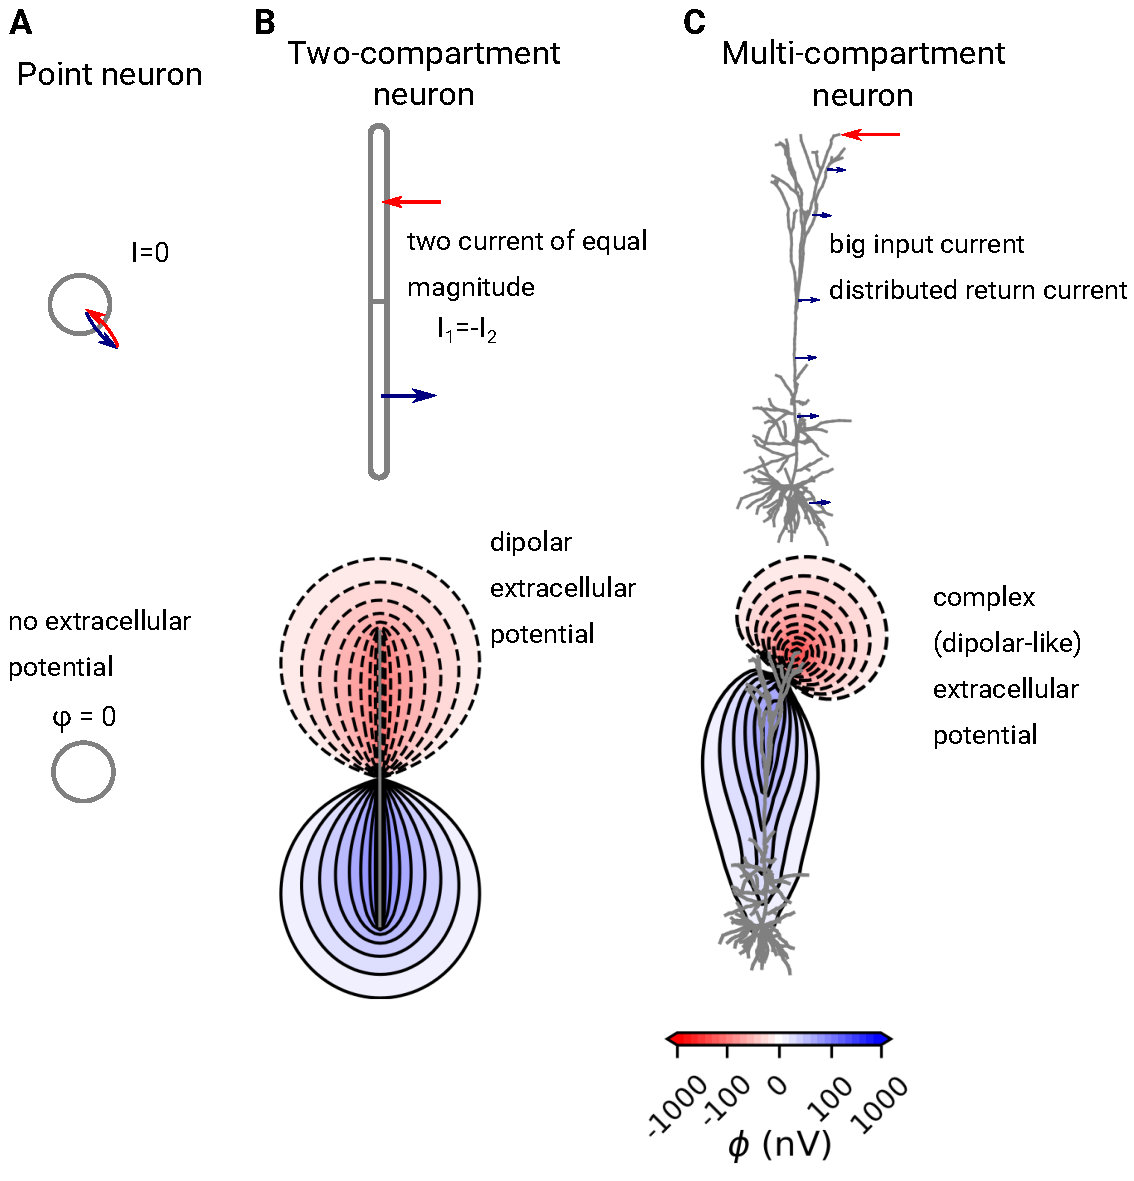
\includegraphics[width=0.6\textwidth]{dipoles}
\end{center}
\caption{\textbf{Effect of current conservation on extracellular potentials.} 
Illustration of synaptic input to three different types of cell models (top row), with the resulting extracellular potentials (bottom row). 
A: Point neurons have no net currents, and therefore cause no extracellular potentials. B: Two-compartment neuron models have two opposite currents
of identical magnitude, and cause dipolar extracellular potentials. C: Multi-compartment neuron models \citep{Hay2011} give rise to extracellular potentials with complex (but mostly dipolar-like) shapes.}
\label{fig:EP_morph_}
\end{figure}


\subsection*{Illustration with two-compartment model}
Consider now a cell model with two cellular compartments. Current conservation, through eq.~\ref{eq:current_conservation}, then implies $I_1 + I_2 = 0$, which in combination with eq.~\ref{eq:VCtheory} gives,
\begin{equation}
 \phi ({\bf r}) = \frac{I_1}{4\pi {\bf |r-r_1|} \sigma} + \frac{-I_1}{4\pi {\bf |r-r_2|} \sigma} = \frac{I_1}{4\pi \sigma}\left ( \frac{1}{{\bf |r-r_1|}} - \frac{1}{{\bf |r-r_2|}}\right ).
\end{equation}
In words, the exact same amount of current that goes into one compartment, goes out of the other, resulting in a current dipole (Fig.~\ref{fig:EP_morph}B).

\subsection*{Illustration with multi-compartment cell model}
For multi-compartment cell models, the situation becomes more complex, but current conservation is still key in shaping extracellular potentials, and ensures that there are no current monopoles. This means that in general neural activity can be expected to cause both negative and positive currents, resulting in both positive and negative extracellular potentials (Fig.~\ref{fig:EP_morph}C).

LFP is low-pass filtered, but note that spikes, like delta-funcitons, have substantial power in low-frequencies.

\subsection*{Correlations boost LFP signals}
Correlations have been demonstrated to play a vital role, and can increase the amplitude of the LFP by orders of magnitude \citep{Linden2011, Leski2013}. The effect is in principle easy to understand (Fig.~\ref{fig:correlation_effect}).

\tvnnote{Could have (i) no figure, (ii) remake figure from Linden et al., (iii) make simple illustration figure of underlying reason for boost?} 

\begin{figure}[ht!]
\begin{center}
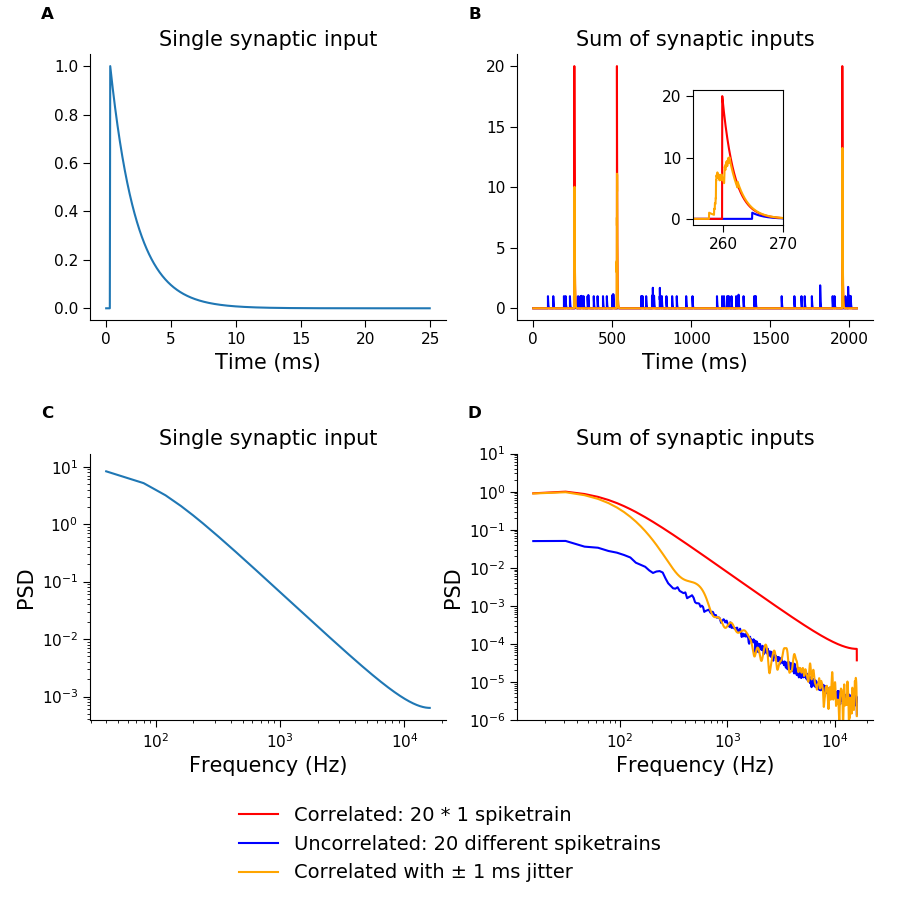
\includegraphics[width=0.5\textwidth]{correlation_jitter}
\end{center}
\caption{\textbf{[Placeholder] Effect of correlation}. Simple illustration of correlation effect. A single instance of a toy ''synaptic input`` (A), is used as a building block for creating ''spike trains`` which are summed into compound signals (B). The ''spike trains`` are either completely uncorrelated, that is, 20 random ''spike trains`` are summed (blue), or completely correlated, that is a single ''spike train`` is summed 20 times (red). Although the blue and red lines had exactly the same number of ''spikes`` (the integral over the signals are identical), the power-spectral density (PSD) of the correlated case is an order of magnitude larger than the uncorrelated case (panel D; red versus blue).}
\label{fig:correlation_effect}
\end{figure}



\subsection{Intrinsic dendritic filtering}
As a thought experiment, imagine a synapse that supplies a cell with a sinusoidal synaptic current. From current conservation we know that this input current must be exactly matched by the ensuing return currents, but how much of the current will leave the membrane in the immediate vicinity of the synapse, and how much will spread through the cell and leave through more distant parts of the membrane? 
%If, for example, the synapse is located on a thin dendritic branch it perhaps seems intuitive that much of the current would move axially within the cell and leave the membrane through the somatic region, where there is much more available membrane area for the current to leave through.
There are basically three ways that currents can leave a cellular compartment. First, there are two types of membrane currents, namely ionic and capacitive.
Ionic currents tend to be on the form $I_i(t)=g \cdot (V(t) - E_{rev})$ for so-called passive currents, while for active currents, $g$ would be time dependent.
The capacitive current at position ${\bf r}$ along the membrane at time $t$, is given by \cite{Koch1999},
\begin{equation}
I_c ({\bf r}, t) = c_m\, \tfrac{dV({\bf r}, t)}{dt},
\end{equation}
with membrane capacitance $c_m$. Lastly, there are axial currents, essentially given by Ohm's law, $I_a = \Delta V / r_a$, where $\Delta V$ is the difference in potential between two neigbouring compartments, and $r_a$ is the resistance between them.

Note that, in contrast to ionic and axial currents, capacitive currents are proportional to the time derivative of the membrane potential, implying that if the hypothetical sinusoidal synapse had a high frequency (say 100-1000~Hz), the
membrane would in effect be ''leakier`` than it would be for a low frequency current (say 1-10~Hz), while the axial resistance would be the same in the two cases. Effectively, this shifts the return currents closer to the input site for higher frequencies than for lower frequencies. 

Passive cell models, that is, cell models without voltage-dependent ion channels (see Sec.~\ref{sec:active}) are linear, meaning that each frequency component can be solved separately, and since all signals can be represented as a sum of sinusoids, this means that as a signal propagates through a cell, it will become increasingly low-pass filtered. This effect is called intrinsic dendritic filtering \citep{Linden2010}, and it can have a substantial influence on extracellular potentials (Fig.~\ref{fig:intrinsic},~\ref{fig:intrinsic2}).
\begin{figure}[ht!]
\begin{center}
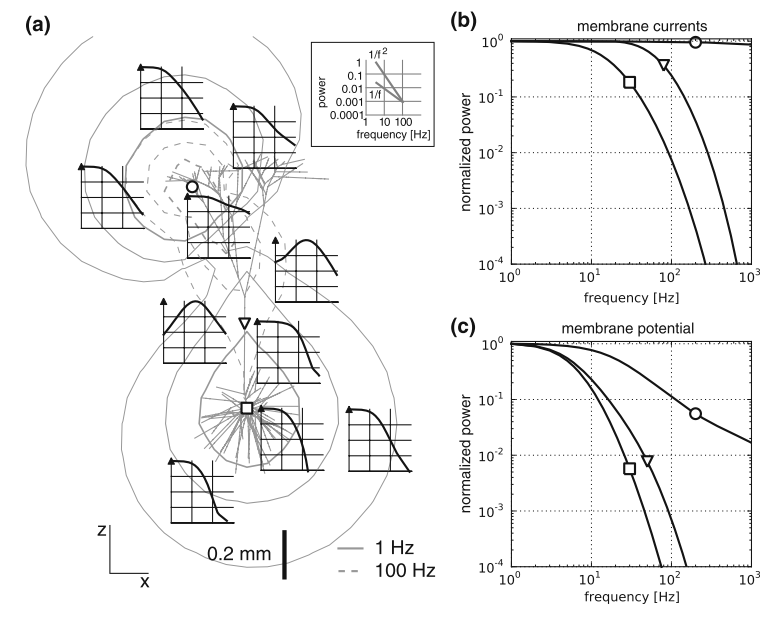
\includegraphics[width=0.5\textwidth]{intrinsic_dendritic_filtering.png}
\end{center}
\caption{\textbf{Intrinsic dendritic filtering} From \cite{Linden2010}.}
\label{fig:intrinsic}
\end{figure}

\begin{figure}[ht!]
\begin{center}
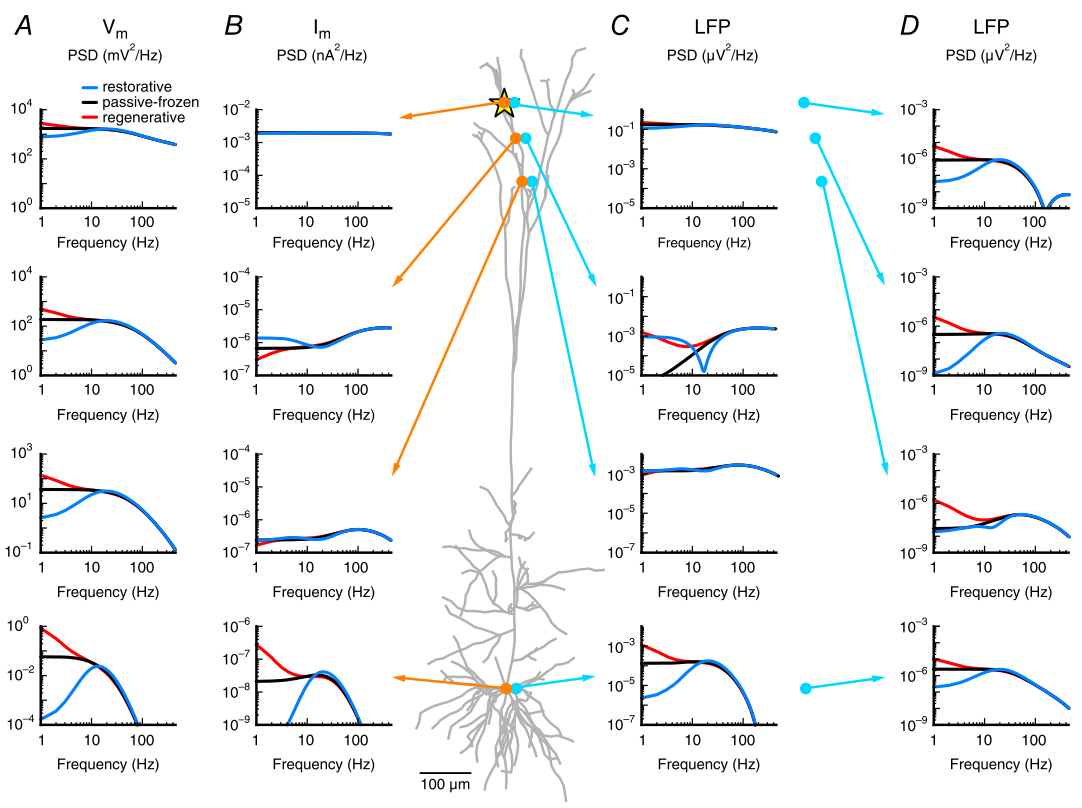
\includegraphics[width=0.8\textwidth]{hay_intrinsic.png}
\end{center}
\caption{\textbf{Intrinsic dendritic filtering} From \cite{Ness2016}.}
\label{fig:intrinsic2}
\end{figure}

\subsection{Old derivation of VC-theory}
\begin{equation}
\nabla^2 \phi = - CSD/\sigma,
\label{eq:trygve}
\end{equation}
where we have introduced the electrical field 

${\bf E}={\bf \nabla} \phi$ \tvnnote{Comment on this? Maxwell -> quasistatic -> cross-product = 0 implies E is gradient of scalar function. Is anything gained by introducing  {\bf E} at all, when we already have $\phi$? Or how about using {\bf E} instead of $\nabla\phi$ from the start?}, and for now assumed that the conductivity, $\sigma$, is a scalar constant. We integrate each side of this equation over a 3D volume,
\begin{equation}
\iiint_V E({\bf r}) \,d^3V =  - \frac{1}{\sigma} \iiint_V \ CSD({\bf r}) \, d^3V.
\label{eq:trygve2}
\end{equation}
If we consider the simplest possible case of a single point current source $I_1$ in ${\bf r}=0$, the right hand side becomes $-I_1/\sigma$. By Gauss' theorem, we can convert the left hand side to a surface integral, and get:
\begin{equation}
\iiint_V E(r) \,d^3V =  \oiint_{S} E(r) \,d^2S = 4\pi r^2 E(r) = 4\pi r^2 \frac{d\phi}{dr} = -\frac{I_1}{\sigma},
\label{eq:trygve3}
\end{equation}
where we have exploited the spherical symmetry of the problem. Finally, integration with respect to $r$ gives us

\subsection{Anisotropy equations}
\begin{equation}
\phi(x,y,z) = \frac{i_e}{4\pi(\sigma_y\sigma_z x^2 + \sigma_x\sigma_z y^2 + \sigma_x\sigma_y z^2)}.
\end{equation}
In cortex, it has been found that the conductivity is in fact about 50 \% higher along the depth axis, that is, parallel to the axis of the pyramidal dendrites \citep{Goto2010}, however, the overall effect of this on extracellular potentials appears quite weak \citep{Ness2015}.

\section{Electrodes}
\tvnnote{Do we want this part?}
\ghnote{I don't. Besides, we probably do not have space to include it.}
\subsection{Size}
Spatial averaging matters, but is relatively easily studied
\subsection{Frequency filtering}
Nelson says no (for recording electrodes) \citep{Nelson2010}

\subsection*{Effect of spikes and active conductances}
\label{sec:active}
\ghnote{Perhaps make this stuff more compact, and not have it as separate subsection?} \tvnnote{I kind off made it more compact, but also expanded the text a bit.}
%Active conductances can affect LFP signals in different ways, for example through the presence of somatic action potentials, dendritic calcium spikes or subthreshold processing of synaptic inputs.
Somatic action potentials are typically not expected to have an important role in shaping cortical LFP signals for several reasons \citep{Einevoll2013, Haider2016}, for example, their very short duration with both positive and negative phases (Fig.~\ref{fig:EP_morph}E) would require extreme synchrony to sum constructively in the LFP, and their high frequency content is to a large degree removed from LFPs during low-pass filtering. 
There are, however, indications that in particular the relatively long-lasting after-hyperpolarization might, at least in some cases, have a role in shaping the LFP, see for example \cite{Reimann2013}.
Note that in the hippocampus the highly synchronized spikes found during sharp wave ripples are expected to strongly shape the LFP \citep{Schomburg2012, Luo2018}. 

It has been demonstrated by \cite{Suzuki2017} that calcium spikes can make sizable contributions to the LFP and ECoG signals, which opens up for exciting research opportunities, given the assumed important physiological role of such calcium spikes\tvnnote{remove?}.

Subthreshold active conductances can also be expected to affect the LFP, and in particular the hyperpolarization-activated cation channel I$_{\rm h}$ might play a key role in this, see \cite{Ness2016, Ness2018}.


\end{document}  
